\newpage
\section{Anti-aliasing filter}
The purpose of the Anti-aliasing filters is to prevent aliasing of the signal during AD-conversion, but also to suppress noise and get a better Signal Noise Ratio (SNR). All sensors in the Rolling Road electrical system have an Anti-aliasing filter.
The filters are not treated as separate blocks due to the fact that the sensors rely on these filters in order to function properly.

%\subsubsection{Calculation of low-pass filter to all the sensors}

\subsection{Design}
The Anti-aliasing filters are made up by analog low-pass filters. The different sensors in the system requires different kinds of anti-aliasing filters and a Matlab script is used to determine the best design for all the sensor.
The script '\textit{ADC\_lowpassFilter}' will automatically find the best components to realized the Anti-aliasing filters from E12 values, and will make sure that it will suppress the aliasing down to the SNR of the ADC. \fxnote{sætning giver ikke mening, Suppres the aliasing down to the SNR? what - TN}
	
\subsubsection*{Torque sensor}
The script below is used to calculate the RC low-pass filter for the Torque Sensor. The script requires the following pieces of information: The sample frequency, the ADC's resolution (number of bits) and the desired cutoff-frequency.

The sample rate is 48000 samples/s and the ADC is using 12 bit to represent the signal. The desired cutoff-frequency is chosen to be the maximum frequency at which the Roll is gonna rotate, if AU2 is chosen as the test object.
\lstset{language=MATLAB}
\begin{lstlisting}
	ADC_fs=48000;
	ADC_N=12;
	fc=444/60; % RPM/60 = 1/s. Max rpm for Rolling Road then testning AU2 444RPM
	
	[R, C, fc_real, M]=ADC_lowpassFilter(ADC_fs, ADC_N, fc, [100*10^-12, 500*10^-9], 100*10^3, 66)
	
	T_AAF_Torque=tf(((1/(R*C))^M)/((s+1/(R*C))^M))
	
	figure;
	bode(T_AAF_Torque);
	legend('show');
	grid on;
\end{lstlisting}
	
The result from the script are the following component-values:	
\begin{equation}
	\begin{split}
	R &= \SI{56}{\kilo\Omega}\\
	C &= \SI{390}{\nano\F}
	\end{split}
\end{equation}
	
And the low-pass filter's transfer function is:
\begin{equation}
	T_{{AAF\_Torque}}(s) = \frac{45.79}{s+ 45.79}
\end{equation}
	
	
\begin{figure}[H]
	\centering
	\includegraphics [width=4in]{Hardware/Pictures/FilterAnalyse_01.eps}
	\caption{Bode plot of the Anti-aliasing filter for the Torque sensor}
	\label{fig:BODE_AAF_Torque}
\end{figure}
	
	
\subsubsection*{Power sensor}
The signal of interest is the average value, because the PWM signal will be seen as noise signal, and must be filtered out, also because else the sample rate have to be around 512 times bigger then PWM frequency. \fxnote{omformulering tak - TN}
	
\begin{lstlisting}
	ADC_fs=52500;
	ADC_N=12;
\end{lstlisting}
	
The following will calculate how much the PWM signal have to be suppressed to meet the requirement of 0.1\% accuracy.
	
\begin{lstlisting}
	Supress_dB=-20*log10(0.001)
\end{lstlisting}

The design will be build based on that the PWM frequency is greater then 2000Hz, and have to suppress the PWM signal 60dB to get an  accuracy of 0.1\%. This can be done with a 2. order low-pass filter 2 decades before 2000Hz this is 20Hz. The PWM signal will be suppressed with 80dB.
	
\begin{lstlisting}
	fc=20;
	
	[R, C, fc_real, M]=ADC_lowpassFilter(ADC_fs, ADC_N, fc, [100*10^-12, 500*10^-9], 100*10^3);
	
	T_AAF_power=tf(((1/(R*C))^M)/((s+1/(R*C))^M))
	
	figure;
	bode(T_AAF_power);
	legend('show');
	grid on;
\end{lstlisting}

The result from the script are: (Note this is a 2. order low-pass filter)
	
\begin{equation}
	\begin{split}
	R &= \SI{68}{\kilo\Omega}\\
	C &= \SI{120}{\nano\F}
	\end{split}
\end{equation}
	
And the transfer function is: 
	
\begin{equation}
	T_{{AAF\_power}}(s) = \frac{15020}{{(s + 122.56)}^{2}}
\end{equation}
	
\begin{figure}[H]
	\centering
	\includegraphics [width=4in]{Hardware/Pictures/FilterAnalyse_02.eps}
	\caption{Bode plot of the Anti-aliasing filter for the power sensor}
	\label{fig:BODE_AAF_power}
\end{figure}

\subsection{Implementation}

Anti-aliasing filter will be realized in the implementation process. To implement the 2. order low-pass filter a buffer is needed, to realize the circuit. As a buffer the IC MCP6004 are used.
	
\subsubsection*{Torque Sensor}
	
\begin{figure}[H]
	\centering
	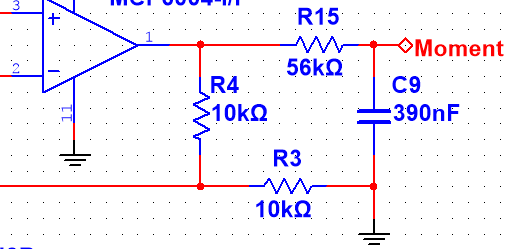
\includegraphics [width=4in]{Hardware/Pictures/AAF_moment.PNG}
	\caption{schematic of the Anti-aliasing filter for the torque sensor}
	\label{fig:schematic_AAF_Torque}
\end{figure}
	
There is not much too add to the torque sensor because it all ready has a buffer, and just a normal RC low-pass filter can be implement, as seen in \vref{fig:schematic_AAF_Torque} where R15 and C9 is the Anti-aliasing filter.
	
\subsubsection*{Power sensor}

\begin{figure}[H]
	\centering
	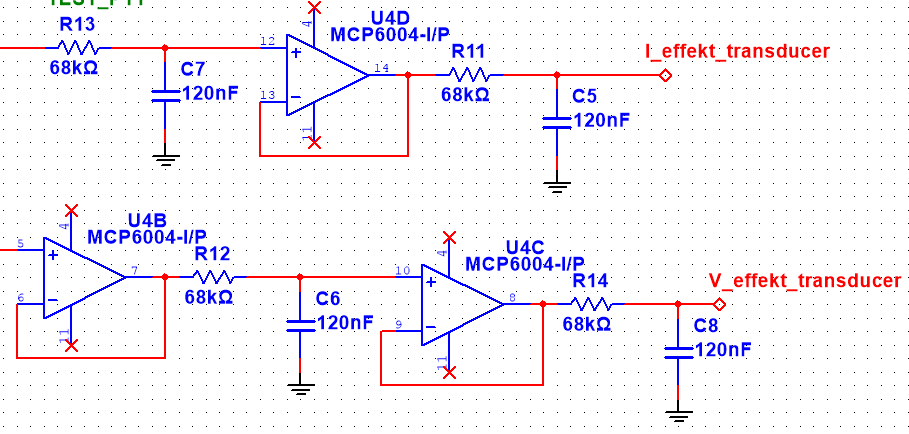
\includegraphics [width=4in]{Hardware/Pictures/AAF_effekt.PNG}
	\caption{schematic of the Anti-aliasing filter for the power sensor}
	\label{fig:schematic_AAF_power}
\end{figure}
	
The power sensor need a couple of buffer to make the 2. order low-pass filters. The reason what the I\_power\_sensor don't need a buffer in front of it is because the sensor all ready have a buffer inside of it.   

\subsection{Unity test}
Text \fxnote{Skal have udført en test når printet er færdigt!}